\section{前処理}
前処理の手法である標準化と正規化にについて述べる.
本実験では,前処理として主に標準化を用い,結果の比較のため正規化も行った.\\
どちらもデータのスケールを揃えるために用いられ,データの重要性を均等に扱ったり,学習の収束を早める効果がある.\\
それぞれの手法の違いは下記の通りである.本研究では,データのスケールが特徴量ごとに異なるため,標準化を用いる.

また,AutoEncoderから生成した特徴量を,標準化するべきか否かは,別途実験により検証する.

\subsection{標準化}

標準化とは,データの平均を0,標準偏差を1にする変換である.
図を\ref{fig:standardization}に示す.
変換式は式\ref{eq:standardization}の通りである.
分布の形状を保ったまま,データのスケールの大小を揃えることができる.
また,偏差を用いるため,外れ値の影響を受けにくいという特徴がある.
本実験で標準化する際は,学習データの平均と分散を用いて,テストデータも標準化する.
これは機械学習モデルを学習した段階では,まだ知らないはずのテストデータの平均と分散を使用できないからである.

\begin{equation}
  \label{eq:standardization}
  x' = \frac{x - \mu}{\sigma}
\end{equation}
なお,$\mu$は平均,$\sigma$は標準偏差である.

\begin{figure}[htbp]
  \centering
  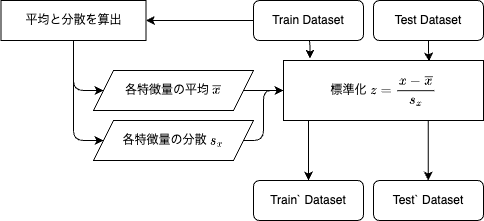
\includegraphics[width=0.6\linewidth]{figures/standardization.png}
  \caption{標準化の流れ}
  \label{fig:standardization}
\end{figure}

\subsection{正規化}

正規化とは,データの最大値を1,最小値を0にする変換である.
図を\ref{fig:normalization}に示す.
変換式は式\ref{eq:normalization}の通りである.
CNNによる画像認識など,データの取りうる値の範囲が一定である場合によく用いられる.

\begin{equation}
  \label{eq:normalization}
  x' = \frac{x - x_{\min}}{x_{\max} - x_{\min}}
\end{equation}
なお,$x_{\min}$は最小値,$x_{\max}$は最大値である.

\begin{figure}[htbp]
  \centering
  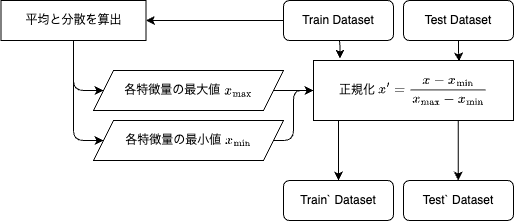
\includegraphics[width=0.6\linewidth]{figures/normalization.png}
  \caption{正規化の流れ}
  \label{fig:normalization}
\end{figure}
